\section{任务三}

本任务使用五组轮密钥，检验四轮 CipherFour 的差分概率在具体密钥下是否保持不变。输入差分和目标输出差分分别为
\[
    \Delta_{in}=0x0001,\qquad \Delta_{out}=0x0010.
\]
每组密钥包含五个 16 比特字：前四个分别在四轮开始时与状态异或，第五个在四轮结束后与状态异或。最后一个密钥字是输出白化密钥，不是第五个 S-P 轮。

\subsection{实验方法}

程序先计算 16 比特状态经过一层 S 盒和 P 置换的查找表。对任一输入状态 $v$，查找表保存
\[
    SP[v]=P(S(v)).
\]
因此，对固定密钥组 $(k_0,k_1,k_2,k_3,k_4)$，四轮加密可写为
\[
    X_0=x,\qquad
    X_{i+1}=SP[X_i\oplus k_i]\quad (i=0,1,2,3),\qquad
    E_k(x)=X_4\oplus k_4.
\]
代码先为全部 $2^{16}$ 个状态构造查找表：
\begin{lstlisting}
for value in range(STATE_SIZE):
    SP_table[value] = P_box(S_box(value))
\end{lstlisting}
再用该表执行四轮加密：
\begin{lstlisting}
state = plainText
for round_index in range(NUMBER_OF_ROUNDS):
    state = SP_table[state ^ keys[round_index]]
return state ^ keys[NUMBER_OF_ROUNDS]
\end{lstlisting}

实验固定随机种子为 \texttt{20260922}，随机生成五组互不相同的密钥。对每组密钥，程序计算全部 $2^{16}$ 个明文的密文，并枚举
\[
    (x,x')=(x,x\oplus 0x0001),\qquad 0\le x<2^{16}.
\]
若密文差分为 $0x0010$，就将匹配数加一。对第 $j$ 组密钥，记匹配数为 $N_j$，则实验频率为
\[
    P_j=\frac{N_j}{2^{16}}.
\]
循环遍历所有 $x$，所以每个无序明文对按正、反两个顺序各统计一次。

\subsection{实验结果}

五组密钥及其统计结果如下。表中密钥字按 $(k_0,k_1,k_2,k_3,k_4)$ 排列，其中 $k_4$ 是四轮后的输出白化密钥。

\begin{table}[H]
    \centering
    \small
    \caption{五组密钥下四轮差分 $0x0001\rightarrow0x0010$ 的统计结果}
    \begin{tabular}{c p{0.55\textwidth} r r}
        \hline
        组别 & 密钥组 $(k_0,k_1,k_2,k_3,k_4)$ & 匹配对数 $N_j$ & 频率 $P_j$ \\
        \hline
        1 & \texttt{[0xB8E5, 0x3463, 0x03F1, 0x26A1, 0x13E1]} & 3080 & 0.0469970703 \\
        2 & \texttt{[0x216F, 0xEAC8, 0xD44F, 0x1EE4, 0x6EA1]} & 3058 & 0.0466613770 \\
        3 & \texttt{[0x4DEC, 0x374E, 0x68DC, 0xC60D, 0x57F9]} & 3076 & 0.0469360352 \\
        4 & \texttt{[0x945E, 0x835B, 0x9F29, 0x33D3, 0xC82A]} & 3054 & 0.0466003418 \\
        5 & \texttt{[0xBC38, 0x20B4, 0x3ACF, 0x3CE6, 0xD29B]} & 3070 & 0.0468444824 \\
        \hline
    \end{tabular}
\end{table}

五组频率的平均值为
\[
    \overline{P}
    =\frac{1}{5}\sum_{j=1}^{5}P_j
    =0.0468078613.
\]

\begin{figure}[H]
    \centering
    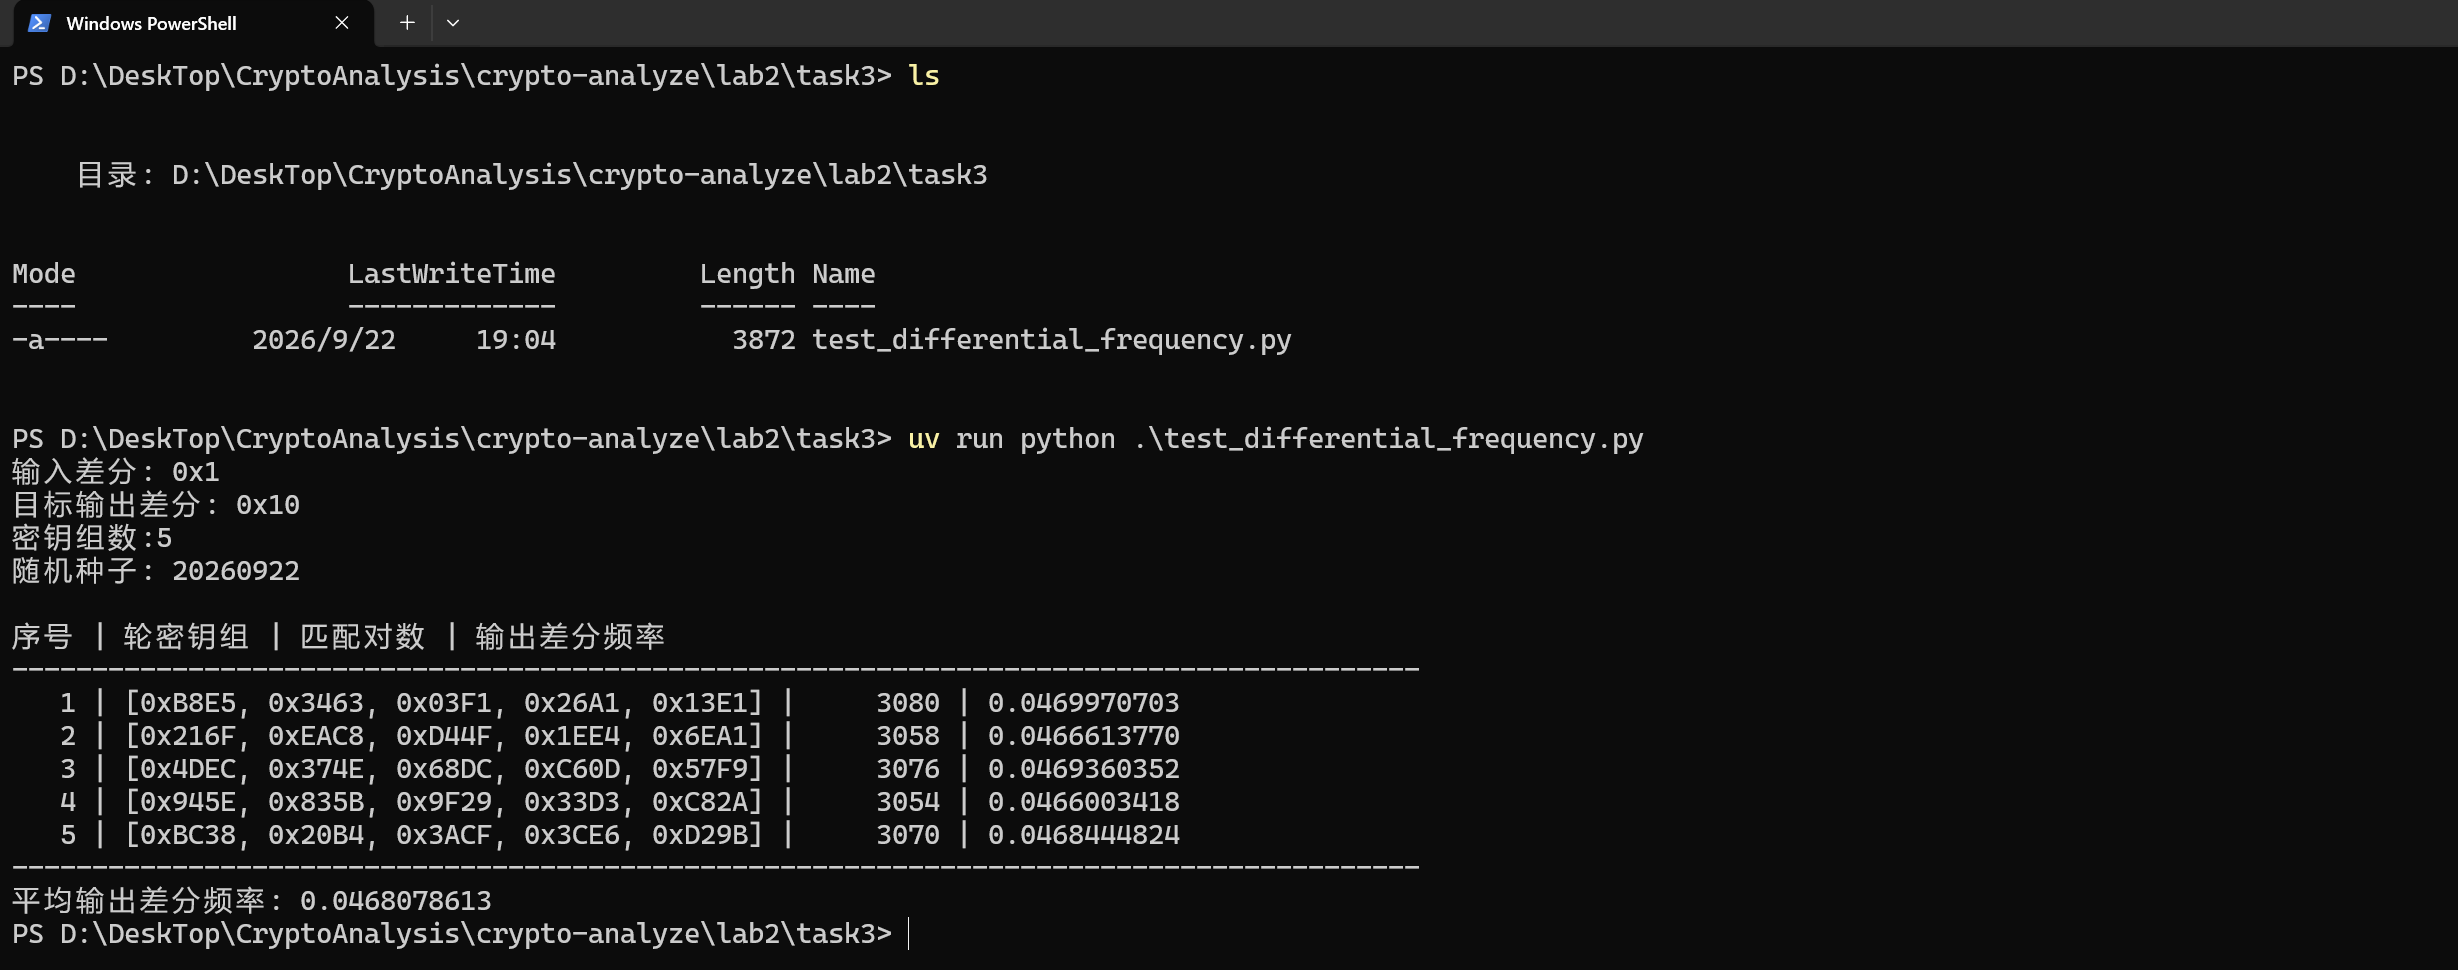
\includegraphics[width = 0.96\textwidth]{figures/task3_different_key.png}
    \caption{五组密钥下的差分频率统计过程与结果}
\end{figure}

五组频率落在 $0.04660$ 到 $0.04700$ 之间，平均约为 $0.04681$。任务一通过 DDT 逐轮传播差分概率，得到 $0.0479736328125$；本任务则对每组固定密钥穷举全部明文对，得到该具体密钥下的精确频率。两者接近但不完全相等，说明固定密钥下的逐轮差分传播并不等同于 DDT 模型给出的概率。
该结果与任务一中的DDT差分概率传播模型、任务二中找到所有4轮差分路线的概率大致等，说明实际运行结果与理论分析非常相近，相互印证了前面几个实验的结果是正确的。

四轮结束后的白化密钥 $k_4$ 对一对密文都执行相同的异或，因此在密文差分中抵消。频率随密钥组变化，来自前四轮密钥对各轮 S 盒输入状态的影响。
